%%%%%%%%%%%%%%%%%%%%%%%%%%%%%%%%%%%%%%%%%%%%%%%%%%%%%%%%%%%%%%%%%%%%%%%%%%%%
%%%%%%%%%%%%%%%%%%%%%%%%%%%%%%%%%%%%%%%%%%%%%%%%%%%%%%%%%%%%%%%%%%%%%%%%%%%%
%%%%%%%%%%%%%%%%%%%%%%%%%%%%%%%%%%%%%%%%%%%%%%%%%%%%%%%%%%%%%%%%%%%%%%%%%%%%

\section{Dynamic Programming | Set 11 (Egg Dropping Puzzle)
  \label{secGFGDPSet11EggDropPuzz}}

\url{http://www.geeksforgeeks.org/dynamic-programming-set-11-egg-dropping-puzzle}

\textbf{Difficulty: 4.3}

The following is a description of the instance of this famous puzzle
involving $n=2$ eggs and a building with $k=36$ floors.

Suppose that we wish to know which stories in a 36-story building are safe
to drop eggs from, and which will cause the eggs to break on landing. We
make a few assumptions:
\begin{itemize}[noitemsep,topsep=0pt]
\item An egg that survives a fall can be used again.
\item A broken egg must be discarded.
\item The effect of a fall is the same for all eggs.
\item If an egg breaks when dropped, then it would break if dropped from a
  higher floor.
\item If an egg survives a fall then it would survive a shorter fall.
\item It is not ruled out that the first-floor windows break eggs, nor is it
  ruled out that the $36$th-floor do not cause an egg to break \rrblue{(this
    implies that we'd have to test the first floor, and the last floor,
    since the last floor may not break the eggs.)}.
\end{itemize}
If only one egg is available and we wish to be sure of obtaining the right
result, the experiment can be carried out in only one way. Drop the egg from
the first-floor window; if it survives, drop it from the second floor
window. Continue upward until it breaks. In the \textbf{worst case}, this
method may require $36$ droppings. Suppose 2 eggs are available. What is the
least number of egg-droppings that is guaranteed to work in all cases.

\rrblue{(By considering the worst case, we can guarantee that it works for
  all cases.  I.e. the least number of drops that would work for the worst
  case is the most number of drops we'll need for other cases.)}?

\rrblue{(For the example above, the worst case we'll need 36 drops (if the
  critical floor is floor 36. Now, if the critical floor is anything lower
  than 36, using max 36 drops would work for all other cases.))}

\textbf{\rrgreen{Recommended: Please try your approach first, before moving
    on to the solution.}}

\RayNotesBegin

We'll add notes from
\url{https://en.wikipedia.org/wiki/Dynamic\_programming#Egg\_dropping\_puzzle}
in case there is something interesting, then we'll continue with our
solution, then onto the GFG solution.

\rrheader{Egg dropping puzzle}

The following is a description of the instance of this famous puzzle
involving $n=2$ eggs and a building with $H=36$ floors:
\begin{quotation}
Suppose that we wish to know which stories in a 36-story building are safe
to drop eggs from, and which will cause the eggs to break on landing (using
U.S. English terminology, in which the first floor is at ground level). We
make a few assumptions:
\begin{itemize}%[noitemsep,topsep=0pt]
\item An egg that survives a fall can be used again.
\item A broken egg must be discarded.
\item The effect of a fall is the same for all eggs.
\item If an egg breaks when dropped, then it would break if dropped from a
  higher window.
\item If an egg survives a fall, then it would survive a shorter fall.
\item It is not ruled out that the first-floor windows break eggs, nor is it
  ruled out that eggs can survive the $36$th-floor windows.
\end{itemize}
If only one egg is available and we wish to be sure of obtaining the right
result, the experiment can be carried out in only one way. Drop the egg from
the first-floor window; if it survives, drop it from the second-floor
window. Continue upward until it breaks. In the worst case, this method may
require $36$ droppings. Suppose $2$ eggs are available. What is the
\textbf{lowest number} of egg-droppings that is \textbf{guaranteed to work
  in all cases}?
\end{quotation}
To derive a dynamic programming functional equation for this puzzle, let the
\textbf{state} of the dynamic programming model be a pair $s=(n,k)$, where
\begin{itemize}%[noitemsep,topsep=0pt]
\item $n$ = number of test eggs available, $n=0,1,2,3,\ldots,N-1$.
\item $k$ = number of (consecutive) floors yet to be tested,
  $k=0,1,2,\ldots,H-1$.
\end{itemize}
For instance, s = (2,6) indicates that two test eggs are available and 6
(consecutive) floors are yet to be tested. The initial state of the process
is $s=(N,H)$ where $N$ denotes the number of test eggs available at the
commencement of the experiment. The process terminates either when there are
no more test eggs ($n=0$) or when $k=0$, whichever occurs first. If
termination occurs at state $s=(n=0,k>0)$ and $k>0$, then the test failed
(since we have no more eggs but still floors to test).

Now, let
\begin{quotation}
$W(n,k)$ = minimum number of trials required to identify the value of the
critical floor under the \textbf{worst-case} scenario given that the process
is in state $s=(n,k)$.
\end{quotation}
Then it can be shown that
\begin{quotation}
\begin{lstlisting}[style=raygeneric]
W(n,k)=1+min{max(W(n - 1, x - 1),
                 W(n,k - x)      ): x = 1, 2, ..., k }
\end{lstlisting}
\end{quotation}
with $W(n,0)=0$ for all $n > 0$ and $W(1,k) = k$ for all $k$. It is easy to
solve this equation iteratively by systematically increasing the values of
$n$ and $k$.

Logic for the above equation:
\begin{enumerate}[label=\textbf{\arabic*.}]
\item If the egg breaks after dropping from the $x$th floor, then we only
  need to check for floors lower than x with the remaining eggs, so the
  problem reduces to $x-1$ floors and $n-1$ eggs.
\item If the egg doesn't break after droppinf from the $x$th floor, then we
  only need o check for floors higher than $x$; so the problem reduces to
  $k-x$ floors with $n$ eggs.
\end{enumerate}
An interactive online facility is available for experimentation with this
model as well as with other versions of this puzzle (e.g. when the objective
is to minimize the \textbf{expected value} of the number of trials.)

\rrheader{Faster DP solution using a different parametrization}

Notice that the above solution takes $\comBigOh{nk^{2}}$ time with a DP
solution. This can be improved to $\comBigOh{nk\log k}$ time by binary
searching on the optimal $x$ in the above recurrence, since $W(n-1,x-1)$ is
increasing in $x$ while $W(n,k-x)$ is decreasing in $x$, thus a local
minimum of $\max(W(n-1,x-1),W(n,k-x))$ is a global minimum.  Also, by
storing the optimal $x$ for each cell in the DP table and referring to its
value for the previous cell, the optimal $x$ for each cell can be found in
constant time, improving it to $\comBigOh{nk}$ time. However, there is an
even faster solution that involves a different parametrization of the
problem:

RRRTODO, okay, the wikipedia entry doesn't provide any new insight, I'll
just do my solution now. But check out the next bit, it's pretty interesting
to come up with a $\comBigOh{n\log n}$ solution.

%Let {\displaystyle k} k be the total number of floors such that the eggs break when dropped from the {\displaystyle k} kth floor (The example above is equivalent to taking {\displaystyle k=37} k=37).
%
%Let {\displaystyle m} m be the minimum floor from which the egg must be dropped to be broken.
%
%Let {\displaystyle f(t,n)} f(t,n) be the maximum number of values of {\displaystyle m} m that are distinguishable using {\displaystyle t} t tries and {\displaystyle n} n eggs.
%
%Then {\displaystyle f(t,0)=f(0,n)=1} f(t,0)=f(0,n)=1 for all {\displaystyle t,n\geq 0} t,n\geq 0.
%
%Let {\displaystyle a} a be the floor from which the first egg is dropped in the optimal strategy.
%
%If the first egg broke, {\displaystyle m} m is from {\displaystyle 1} 1 to {\displaystyle a} a and distinguishable using at most {\displaystyle t-1} t-1 tries and {\displaystyle n-1} n-1 eggs.
%
%If the first egg did not break, {\displaystyle m} m is from {\displaystyle a+1} a+1 to {\displaystyle k} k and distinguishable using {\displaystyle t-1} t-1 tries and {\displaystyle n} n eggs.
%
%Therefore, {\displaystyle f(t,n)=f(t-1,n-1)+f(t-1,n)} f(t,n)=f(t-1,n-1)+f(t-1,n).
%
%Then the problem is equivalent to finding the minimum {\displaystyle x} x such that {\displaystyle f(x,n)\geq k} f(x,n)\geq k.
%
%To do so, we could compute {\displaystyle \{f(t,i):0\leq i\leq n\}} \{f(t,i):0\leq i\leq n\} in order of increasing {\displaystyle t} t, which would take {\displaystyle O(nx)} O(nx) time.
%
%Thus, if we separately handle the case of {\displaystyle n=1} n=1, the algorithm would take {\displaystyle O(n{\sqrt {k}})} O(n{\sqrt {k}}) time.
%
%But the recurrence relation can in fact be solved, giving {\displaystyle f(t,n)=\sum _{i=0}^{n}{\binom {t}{i}}} f(t,n)=\sum _{i=0}^{n}{\binom {t}{i}}, which can be computed in {\displaystyle O(n)} O(n) time using the 
%
%identity {\displaystyle {\binom {t}{i+1}}={\binom {t}{i}}{\frac {t-i}{i+1}}} {\binom {t}{i+1}}={\binom {t}{i}}{\frac {t-i}{i+1}} for all {\displaystyle i\geq 0} i\geq 0.
%
%Since {\displaystyle f(t,n)\leq f(t+1,n)} f(t,n)\leq f(t+1,n) for all {\displaystyle t\geq 0} t\geq 0, we can binary search on {\displaystyle t} t to find {\displaystyle x} x, giving an {\displaystyle O(n\log k)} O(n\log k) algorithm.

\qasepline{}

I've found a much better explanation on
\url{https://brilliant.org/wiki/egg-dropping}:

\textbf{Egg dropping} refers to a \emph{class of problems} in which it is
important to find the correct response without exceeding a (low) number of
certain failure states. In a toy example, there is a tower of $n$ floors,
and an egg dropper with $m$ ideal eggs. The physical properties of the ideal
egg is such that it will shatter if it is dropped from floor $n^*$ or above,
and will have no damage whatsoever if it is dropped from floor $n^*-1$ or
below. The problem is to find a strategy such that the egg dropper can
determine the floor $n^*$ in as few egg drops as possible. This problem has
many applications in the real world such as avoiding a call out to the slow
HDD, or attempting to minimize cache misses, or running a large number of
expensive queries on a database.

\rrheader{Contents:}

\begin{itemize}%[noitemsep,topsep=0pt]
\item $2$ Eggs, $100$ Floors (see \pagecref{rrED2Eggs100Floors})
\item $2$ Eggs, $k$ Floors (see \pagecref{rrED2EggskFloors})
\item $N$ Eggs, $k$ Floors (see \pagecref{rrEDNEggskFloors})
\item Recursive Solution (see \pagecref{rrED2RecurSol})
\item DP Solution (see \pagecref{rrEDDPSol})
\item Working with Binomials (see \pagecref{rrEDWorkingWithBinom})
\item A Better Approach (see \pagecref{rrEDABetterApproach})
\item See also (see \pagecref{rrEDSeeAlso})
\item Complexity (see \pagecref{rrEDComplexity})
\end{itemize}

\rrheader{$2$ Eggs, $100$ Floors\label{rrED2Eggs100Floors}}

Suppose you have two eggs and you want to determine from which floors in a
one hundred floor building you can drop an egg such that is doesn't break.
You are to determine the \textbf{minimum number of attempts} you need in
order to find the critical floor in \textbf{the worst case} while using the
best strategy.
\begin{itemize}%[noitemsep,topsep=0pt]
\item If the egg doesn't break at a certain floor, it will not break at any
  floor below.
\item If the eggs breaks at a certain floor, it will break at any floor
  above.
\item The egg may break at the first floor.
\item The egg may not break at the last floor.
\end{itemize}
One would be tempted to solve this problem using binary search, but actually
this is not the best strategy, and you will see why. Try to work it out
yourself and answer this question, or read on to see a detailed explanation
of the problem.

\begin{quotation}\color{darkgray}
You are asked to find the highest floor of 100-story building from which an
egg can be dropped without breaking. You have two eggs to test-drop from the
building, and you can continue to drop your eggs until they break.

From which floor should you drop your first egg to optimize your chances of
dropping the eggs as few times as possible?
\end{quotation}
Using binary search, you would have to drop the first egg from the $50$th
floor. If it doesn't break, you would drop the same egg from the $75$th and
so on; in the best case scenario you would be able to cover all floors with
$7$ drops ($\log_2 100 = 6.64$).

But what if the egg broke in your first attempt, i.e. in the $50$th floor?
If this happens, you are obligated to drop the remaining egg from each floor
until finding $n^*$, which has the potential for $49$ drop tests, which is
$\comBigOh{n}$.

Remember, the problem is to determine the critical floor $n^*$, so you can't
let your last egg break before finding it. Dropping your last egg from the
$25$th floor would be quite risky, if it broke you wouldn't be able to
determine the critical floor. It is clear that binary search is not the
optimal solution. Knowing that, what is the best strategy? From which floor
should you start? What's the minimum number of drops you would have to do in
the worst case while using the best strategy?

Starting from the $14$th floor is the best strategy because, as we will
show, the number of attempts in the worst case is always 14.
\begin{itemize}%[noitemsep,topsep=0pt]
\item What if the first egg breaks at floor $14$?

If the first egg breaks at the $14$th floor, then we should check the first
floor, then the second one, until the $13$th floor. Doing this the total
number of attempts would be $14$.
\item What if it doesn't break? 

Then you should check the $27$th floor. Why? Because if it breaks, you would
have to check all the floors from $15$th until the $26$th one (thirteen
floors), which keeps the total number of attempts at $14$ (first attempt at
the $14$th floor, second at the $27$th floor, and the twelve remaining drops
from the $15$th floor until the $26$th floor).
\end{itemize}

And if it doesn't break, you would have to check the $39$th floor; if it
breaks you would have to check all the floors from the $28$th until $38$th
the one. (Remember, one attempt at the $14$th floor, the second attempt at
the $27$th floor, the third attempt at the $39$th floor, and the $11$
remaining attempts at the floors $\brce*{28,29,30,31,32,33,34,35,36,37}$ and
$38$, totalling $14$ attempts in this case.)

Using the same reasoning, you should check the $50$th floor, the $60$th, the
$69$th, the $77$th, the $84$th, the $90$th, the $94$th, the $99$th and
finally the $100$th one. See? Using this strategy you would cover all the
floors and the number of attempts would never be greater than $14$, even in
the worst cases (see table1).

\begin{figure}
\centering
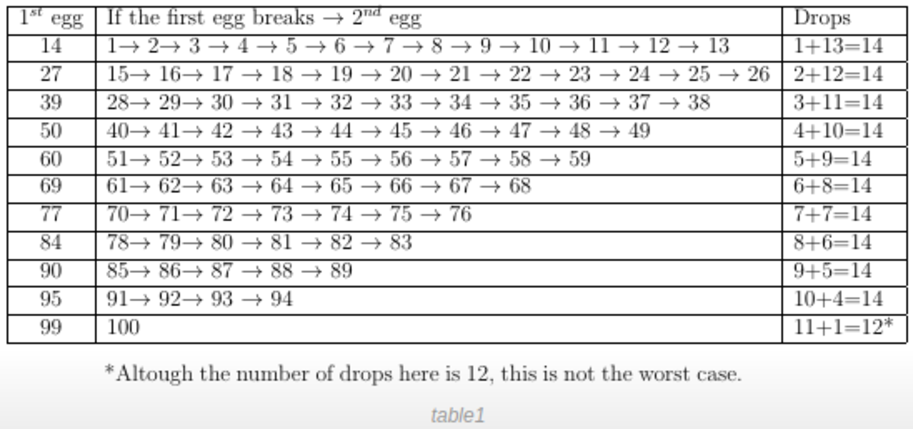
\includegraphics[width=0.8\textwidth]{Images/figBrilliantEggDropTab}
%\caption[]{}
%\label{figBrilliantEggDropTab}
\end{figure}

Using other strategies, like the binary search, fewer attempts would be
required in some cases (like in our first example), but it would require a
high number of attempts in the worst case (in our second example, where the
egg broke in the $50$th floor and $50$ drops were necessary in the worst
case).

Therefore, we can conclude that using another strategy you would need more
than $14$ attempts in the worst case.

\rrheader{$2$ Eggs, $k$ Floors\label{rrED2EggskFloors}}

Now let's try to find a solution for the case where you have $2$ eggs and a
building with $k$ floors.

A good way to start this problem is to ask ``Are we able to cover all the
floors with $x$ drops?''

Suppose that in the best strategy, the number of drops in the worst case is
$x$. Then, you should start at the $x$th floor, because if the egg breaks,
you will have to check floors $1,2,3,\ldots,x-2$ and $x-1$, so the total
number of drops will be $x$. If it doesn't break, you will have to check the
$(x+(x-1))$th floor. If the egg breaks, you will have to check the floors
$x+1$, $x+2$, $\ldots$, $(x+(x-1)-1)$. Hence, the number of drops will be
$(x+(x-1)-1)-(x+1)+1+2=x$.

If you're confused about the last equation, consider this: We test at $14$th
floor and it doesn't break, so next we test at $14+(14-1)=14+13=27$th floor,
if it breaks, we'll have to test from $14+1$, $14+2$, $\ldots,$
$14+(14-1)-1=14+12=26$. Hence, the number of drops will be
$(14+(14-1)-1)-(14+1)+1+2=14$..... actually, I still dunno where the two +1
comes from. I should just do $(14+(14-1)-1)-14 + 2=14$, makes more sense to
me.

Do you realize what we are doing? Based on the assumption that the number of
drops will always be $x$ in the worst case, we find the floors where we
should drop the egg. The crucial point here is understanding that we are not
trying to find the minimum number of drops knowing the best strategy;
actually, we are trying to find the best strategy supposing that the minimum
number of drops is $x$, and we have to determine if covering all the floors
using at most attempts is possible or not.

We can find an analytical solution to this problem:

\begin{mdframed}[style=mdfNOTE,
frametitle={Example}]

Suppose the minimum number of attempts in the worst case, while using the
best strategy, is $x$. In our attempt, we will drop the egg at the $x$th
floor, covering $x$ floors, then we will drop it at the $(x+(x-1))$th floor,
covering $x-1$ floors, and the third drop would be at the
$(x+(x-1)+(x-2))$th floor, covering $x-2$ floors. We can see that using this
strategy we would cover
\begin{equation*}
x+(x-1)+(x-2)+(x-3)+\cdots+2+1=\frac{x(x+1)}{2}
\end{equation*}
floors.

If we are able to cover $\frac{x(x+1)}{2}$ floors using this strategy and
the building has $k$ floors, we just have to find the minimum value of $x$
such that
\begin{equation*}
\frac{x(x+1)}{2}\geq k.
\end{equation*}
Hence,
\begin{equation*}
x^2+x-2k = 0 \implies x = \frac{-1\pm\sqrt{1+8k}}{2}.
\end{equation*}
But  must be an integer, implying
\begin{equation*}
x=\ceil*{\frac{-1\pm\sqrt{1+8k}}{2}}.
\end{equation*}
In our first example, $k=100$, so plugging it into the previous equation
gives $\ceil*{13.65}=14$.

\end{mdframed}

\rrheader{$N$ Eggs, $k$ Floors\label{rrEDNEggskFloors}}

Suppose you have $N$ eggs and you want to determine from which floors in a
$k$-floor building you can drop an egg such that is doesn't break. You are
to determine the minimum number of attempts you need in order find the
critical floor in the \textbf{worst case} while using the best strategy. Now
the problem is a bit more complicated because we must find a general
solution for any number of eggs and floors. There are three different
solutions:
\begin{itemize}%[noitemsep,topsep=0pt]
\item \textbf{The recursive solution:} \\
This solution is more straightforward and can be implemented with ease, but
it is also the slowest one. Using this solution on programming contests is
not advisable due to its bad performance.
\item \textbf{The dynamic programming solution:} \\
This solution is similar to the previous one, but it's faster and may be
used to solve the problem for medium or small values of $k$ and $N$.
\item \textbf{A solution that combines both binary search and recursion:} \\
This is the faster one, and once the strategy is understood, it is rather
easy to implement.
\end{itemize}

\rrheader{Recursive Solution\label{rrED2RecurSol}}

Imagine the following situation: you have $n$ eggs and $h$ consecutive
floors yet to be tested, and afterward you drop the egg at floor $i$ in this
sequence of $h$ consecutive floors:
\begin{itemize}%[noitemsep,topsep=0pt]
\item If the eggs breaks: \\
The problem reduces to $n-1$ eggs and $i-1$ remaining floors.
\item If it doesn't break: \\ The problem reduces to $n$ eggs and $h-i$
  remaining floors. This is an important point. \textbf{The floors we want
    to test aren't important; in fact, \emph{the number of remaining floors
      is what matters}.} For example, testing the floors between 1 and 20
  (both 1 and 20 included) would require the same number of drops to test
  the floors between 21 and 40, or between 81 and 100. In all three
  situations, we tested 20 floors.
\end{itemize}

Now we can define a function $W(n,h)$ that computes the minimum number of
drops required to find the critical floor in the worst case scenario,
\textbf{whilst using the best strategy}.

We can codify the above findings to find the following recursion for
determining $W(n,h)$:

\begin{mdframed}[style=mdfNOTE,
frametitle={Definition}]

\rrheader{Recursion for the egg dropping puzzle:}

\begin{equation*}
W[n,h]=1+\min\paren*{\max \paren*{W(n-1,i-1),W(n,h-i)}}.
\end{equation*}

\end{mdframed}
(Pay attention: $n$=current number of eggs, $N$=total number of eggs,
$h$=number of consecutive floors that still have to be tested, $k$=number of
floors in the building.)

The basis cases are as follows:
\begin{itemize}%[noitemsep,topsep=0pt]
\item Because we need $h$ drops if only $1$ egg remains, $W(1,h) = h$.
\item Because we need only one drop to test one floor, regardless of the
  number of eggs, $W(n,1) = 1$.
\item Because $0$ floors requires no drops, $W(n,0)=0$.
\end{itemize}

\begin{figure}
\centering
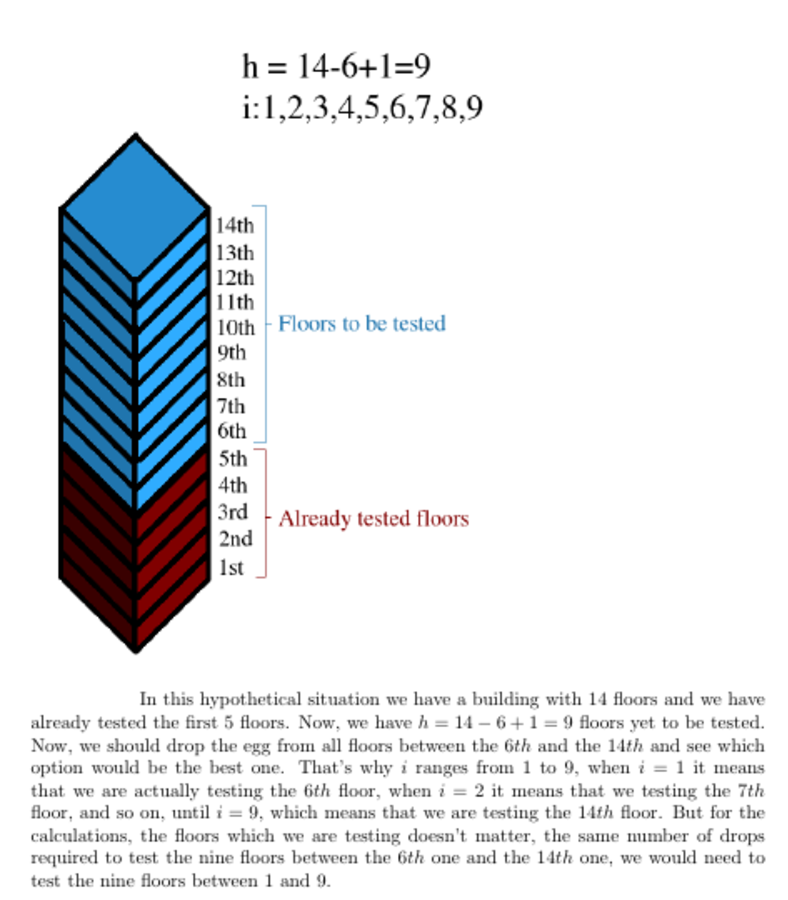
\includegraphics[width=0.9\textwidth]{Images/figBrilliantEggDropTower.ps}
%\caption[]{}
%\label{figBrilliantEggDropTower.ps}
\end{figure}

The pseudo-code for this algorithm is given by
\begin{lstlisting}[style=pseudostyle]
def drops(n,h):
  if(n == 1 or k == 0 or k == 1):
    return k
  end if

  minimum = infty

  for x = 1 to h:
    minimum = min(minimum, 
                  1 + max(drops(n - 1, x - 1), drops(n, h - x))
                  )
  end for

  return minimum
\end{lstlisting}
C++ code that uses the recursive solution:
\begin{lstlisting}[style=raycppnewsnippet]
#include <iostream>
#include <limits.h>

using namespace std;

//Compares 2 values and returns the bigger one
int max(int a,int b) {
  int ans=(a>b)?a:b;
  return ans;
}

//Compares 2 values and returns the smaller one
int min(int a,int b){
  int ans=(a<b)?a:b;
  return ans;
}

int egg(int n,int h){

  //Basis case
  if(n==1) return h;
  if(h==0) return 0;
  if(h==1) return 1;

  int minimum=INT_MAX;

  //Recursion to find egg(n,k). The loop iterates i: 1,2,3,...h
  for(int x=1;x<=h;x++) 
    minimum=min(minimum,
                (1+max(egg(n,h-x),
                       egg(n-1,x-1)
                      )
                 )
                );

    return minimum;
}

int main()
{
  int e;//Number of eggs
  int f;//Number of floors

  cout<<"Egg dropping puzzle\n\nNumber of eggs:";

  cin>>e;

  cout<<"\nNumber of floors:";

  cin>>f;

  cout<<"\nNumber of drops in the worst case:"<<egg(e,f);

  return 0;
}
\end{lstlisting}

\qasepline{}

Here's my attempt, code found in\\
\path{src/DynamicProgramming/rrrGFGDPSet11EggDrop.cpp}
\begin{lstlisting}[style=raycppnewsnippet]
// n - number of eggs
// h - number of floors to be tested
int eggDropRecur(int n, int h)
{
  // Base cases:
  // If there is one egg (n=1) and some floors (h>0), then we always need
  // to test every floor
  if(n==1 && h>0) return h;

  // If there are no floors to be tested (h=0), no drops are required.
  if(h==0) return 0;

  // If there is one floor to be tested, we need 1 drop.
  if(h==1) return 1;

  // Now, we test all floors from x=[1..h].
  // Each drop will give two subproblems:
  //   one for the lower half (if egg breaks)-> x-1 floors to test
  //   one for the upper half (if egg doesn't break)-> h-x floors to test
  // we take the max of the result of the two subproblems 
  // (to get the worst case answer)
  // However, we take the min over all droppings, since we do want the 
  // minimum dropping over the worst case.
  int minimum = std::numeric_limits<int>::max();
  for(int x = 1; x<=h; ++x)
  {
    minimum = std::min(minimum,
                       (1+std::max(eggDropRecur(n-1,x-1), // egg broke
                                   eggDropRecur(n  ,h-x)) // egg no break
                       )
                      );
  }
  return minimum;
}
\end{lstlisting}

\qasepline{}

\rrheader{DP Solution\label{rrEDDPSol}}

The previous solution is very slow, and the same function is called more
than once, which is not necessary. However, due to its overlapping
subproblems, and to its optimal substructure property (we can find the
solution to the problem using the subproblem's optimal solutions), we can
solve the problem via dynamic programming.

We can avoid recalculation of the same subproblems by memoizing the function
egg(n,h) with a two-dimensional array \ctt{numdrops[n][h]}. Then, we just
have to fill it up.

Here's the pseudocode:
\begin{lstlisting}[style=pseudostyle]
def solvepuzzle(N,k):
  for i = 1 to N
    numdrops(i,1) = 1
    numdrops(i,0) = 0
  end for

  for i=1 to k
    numdrops(1, i) = i
  end for

  for i = 2 to N
    for j = 2 to k 

      numdrops[i][j] = infty
      minimum = infty

      for x = 1 to j
        minimum = min(minimum, 
                      1 + max(numdrops(i-1,x-1),numdrops(i,j-x))
                     )
      end for

      numdrops[i][j] = minimum

    end for
  end for

  return numdrops(N,k)
\end{lstlisting}
C++ code:
\begin{lstlisting}[style=raycppnewsnippet]
#include <iostream>
#include <limits.h>

using namespace std;

//Compares 2 values and returns the bigger one
int max(int a,int b) {
  int ans=(a>b)?a:b;
  return ans;
}

//Compares 2 values and returns the smaller one
int min(int a,int b){
  int ans=(a<b)?a:b;
  return ans;
}

int solvepuzzle(int n,int k){

  int numdrops[n+1][k+1];
  int i,j,x;

  for(i=0;i<=k;i++) numdrops[0][i]=0;
  for(i=0;i<=k;i++) numdrops[1][i]=i;
  for(j=0;j<=n;j++) numdrops[j][0]=0;

  //This loop fills up the matrix
  for(i=2;i<=n;i++){
    for(j=1;j<=k;j++){

      //Defines the minimum as the highest possible value
      int minimum=INT_MAX;

      //Evaluates 1+min{max(numeggs[i][j-x],numeggs[i-1][x-1])), for x:1,2,3...j-1,j}
      for(x=1;x<=j;x++) minimum=min(minimum,(1+max(numdrops[i][j-x],numdrops[i-1][x-1])));


      //Defines the minimum value for numeggs[i][j]
      numdrops[i][j]=minimum;
    }

  }

  cout<<"\nArray:\n\n";

  //Prints numeggs
  for(i=0;i<=n;i++){
    for(j=0;j<=k;j++){
      cout<<numdrops[i][j]<<" ";
     }
     cout<<"\n";
  }

  cout<<"\nNumber of trials in the worst case using the best strategy:\n";

  return numdrops[n][k];
}

int main()
{
  int e;//Number of eggs
  int f;//Number of floors

  cout<<"Egg dropping puzzle\n\nNumber of eggs:";

  cin>>e;

  cout<<"\nNumber of floors:";

  cin>>f;

  cout<<solvepuzzle(e,f);

  return 0;
}
\end{lstlisting}

\qasepline{}

I will do bottom up. First, we need a table to store the results in a table
$dp[n+1][k+1]$, where $n=$number of eggs and $k=$number of floor in the
building. We need $+1$ since we're including $0$ eggs and floors. Thus,
$dp[n,k]$ represents the min. number of drop in the worst case for $n$ eggs
and $k$ floors.

First we fill in the base case: For $W(n,k)$, recall:
\begin{itemize}%[noitemsep,topsep=0pt]
\item One egg: $W(n=1,k)=k$.
\item One floor: $W(n,k=1)=1$.
\item Zero floor: $W(n,k=0)=0$.
\end{itemize}
\begin{tabular}{|c|c|c|c|c|c|}\hline
\diagbox{$n$}{$k$}&\textbf{0}&\textbf{1}&\textbf{2}&\textbf{3}&\textbf{4}\\\hline
\textbf{0}&0&1&&&\\\hline 
\textbf{1}&0&1&2&3&4\\\hline
\textbf{2}&0&1&&&\\\hline
\textbf{3}&0&1&&&\\\hline
\textbf{4}&0&1&&&\rrred{(X)}\\\hline
\end{tabular}\\
Now, the recursive call is:
\begin{lstlisting}[style=raycppnewsnippet]
for i=[2..n]
  for j=[2..k]
    for x = [1..j]
      eggDropRecur(i-1,x-1) // egg broke
      eggDropRecur(i  ,j-x) // egg no break
\end{lstlisting}
For now, we will assume that we work in row major order. This may change
depending on the dependencies, for example, if we have:
\begin{equation*}
dp[i,j] = [i,i-1]
\end{equation*}
then it'll make sense to work down the columns first, since each
\ctt{dp[i,j]} depends on the one above it. For 
\ctt{eggDropRecur(i-1,j-1)}, we're getting the solution for \ctt{[i,j]} from
the top left cell, so working in row major order works. What about
\ctt{eggDropRecur(i,j-x)}? Well, we're working on the same row as
\ctt{[i,j]}, but what is \ctt{j-x}? Let's work this out:
\begin{lstlisting}[style=raygeneric]
j=2, x=[1, 2]
j-x:    1  0

j=3, x=[1, 2, 3]
j-x:    2  1  0

j=4, x=[1, 2, 3, 4]
j-x:    3  2  1  0
\end{lstlisting}
So as you can see, each $j$ depends on only previous $j$'s (as opposed to
just the one previous $j$). Thus, it is actually okay to go in row major
order all the way! In fact, it is necessary, because to do (look at the
table \ctt{dp} whilst doing this, it makes more sense), let $i=2$ (the first
row we have to calculate) and move across the columns ($j=$):
\begin{itemize}[noitemsep,topsep=0pt]
\item $(2,2)$, we need the solutions from $(2,1)$ and $(2,0)$, which are
  given by the base case (see the table above).
\item $(2,3)$, we need the solutions from $(3,2)$, $(3,1)$ and $(3,0)$
\end{itemize}
Thus, we must go from left to right!  To do We can do this easily! Let's
code up the DP version!

Here's my attempt, code found in\\
\path{src/DynamicProgramming/rrrGFGDPSet11EggDrop.cpp}
\begin{lstlisting}[style=raycppnewsnippet]
// n - number of eggs
// k - number of floors in the building.
int eggDropDP(const int n, const int k)
{
  // table to store results
  // rows = num eggs
  // column = num floors to be tested.
  vector<vector<int>> dp(n+1,vector<int>(k+1,0));
//  print_2dvec(dp,"initial dp:\n","\n");

  // base cases:
  // 1) If there is one egg (n=1), the required number of drops is the same
  // as the number of floors to be tested W(n=1,k)=k, i.e.:
  //   0 1 2 3 4
  //   ---------
  // 0|
  // 1|0 1 2 3 4
  // 2|
  // 3|
  // 4|
  for(int j=0; j <= k; ++j)
  {
    dp[1][j]=j;
  }
//  print_2dvec(dp,"n=1 dp:\n","\n");

  // Base case 2) If there are no floors (k=0), num drops=0
  //              If there is one floor (k=1), num drops=1
  // So we have
  //   0 1 2 3 4
  //   ---------
  // 0|0 1
  // 1|0 1 2 3 4
  // 2|0 1
  // 3|0 1
  // 4|0 1
  for(int i=0; i<=n; ++i)
  {
    dp[i][0]=0;
    dp[i][1]=1;
  }
//  print_2dvec(dp,"k=0 or 1 dp:\n","\n");


	// Fill rest of the entries in table using optimal substructure
	// property
  for (int i = 2; i <= n; i++)
  {
    for (int j = 2; j <= k; j++)
    {
      dp[i][j] = INT_MAX;
			for (int x = 1; x <= j; x++)
			{
				int res = 1 + std::max(dp[i-1][x-1], dp[i][j-x]);
				if (res < dp[i][j])
					dp[i][j] = res;
			}
		}
	}

  // Now loop through the rows (num of eggs)
  for(int i=2; i <= n; ++i)
  {
    // Now loop through the number of floors.
    for(int j=2; j<= k; ++j)
    {
      // Now we drop the egg from each floor from x=[1..j]
      dp[i][j] = std::numeric_limits<int>::max();
      for(int x=1; x<=j; ++x)
      {
        dp[i][j] = std::min(dp[i][j],(1+std::max(dp[i-1][x-1],
                                                 dp[i][j-x])
                                     )
                           );
      }
    }
  }

//  print_2dvec(dp,"dp:\n","\n");
  return dp[n][k];
}
\end{lstlisting}

\rrheader{Working with Binomials\label{rrEDWorkingWithBinom}}

Before advancing to the next section we must see some useful mathematical
relations related to binomials.

We know that
\begin{equation*}
C^m_k=C(n,k)=\binom{n}{k}=\frac{n!}{(n-k)!k!}
\end{equation*}
We also know that the Pascal triangle is

%\begin{figure}
%\centering
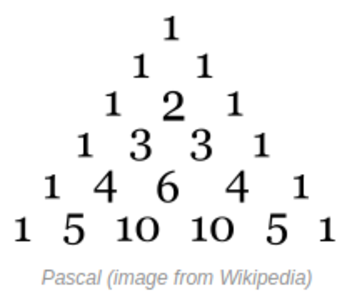
\includegraphics[width=0.2\textwidth]{Images/figBrilliantEggDropPascalsTri}
%\caption[]{}
%\label{figCXNX}
%\end{figure}

And we can easily find a recursion if we write the Pascal triangle in this
way:

%\begin{figure}
%\centering
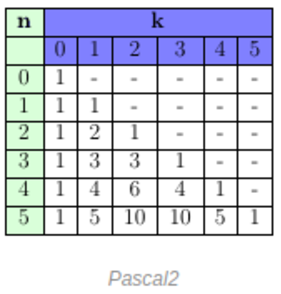
\includegraphics[width=0.3\textwidth]{Images/figBrilliantEggDropPascalsTri2}
%\caption[]{}
%\label{figCXNX}
%\end{figure}

By looking at the table or by a simple mathematical proof we get the
following recurrence:
\begin{equation*}
C(n,k)=C(n-1,k)+C(n-1,k-1),
\end{equation*}
And the basis cases are
\begin{equation*}
C(n,0)=\frac{n!}{(n-0)!0!}=1 \text{ and } C(n,n)=\frac{n!}{(n-n)!n!}=1
\end{equation*}

\rrheader{A Better Approach\label{rrEDABetterApproach}}

RRRTODO - I've given up on this for now. But it uses an identity in the code
at the end, which can be found in the wikipedia article:
\url{https://en.wikipedia.org/wiki/Dynamic\_programming#Egg\_dropping\_puzzle}


With this knowledge in hand, let's define a function $f(d,n)$ that
represents the \textbf{number of floors} we can cover using $n$ eggs and
with $d$ remaining drops.  If the egg breaks we will be able to cover
$f(d-1,n-1)$ floors, otherwise we'll be able to cover $f(d,n-1)$ floors.
Hence, the total number of floors we will be able to cover is
\begin{equation*}
f(d,n)=1+f(d-1,n-1)+f(d-1,n).
\end{equation*}

We must find a function $f(d,n)$ that's a solution for this recursion.
First, we will define an auxiliary function $g(d,n)$:
\begin{equation*}
g(d,n) = f(d,n+1)-f(d,n)
\end{equation*}

Plugging it into our first equation gives
This is precisely the same recursion that we saw in the previous section, and thus the function  can be written as
But we have a problem:  is 0 for every
, as well as , according to the relation between  and . However, a contradiction occurs when  because . But  should be  for every ! We can fix this problem by defining  as follows:
And the recursion is still valid (you can check it by yourself!).

Now, using a telescopic sum for , we can write it as
We know that , and therefore

And we also know that
Hence,
Finally,
Now that we have a nice formula for  how can we find the minimum number of drops?

It's simple! We know that  is the number of floors we can cover in the building with  floors using  eggs and no more than  drops in the worst cases. We simply have to find a value for  such that
Using our last formula,

This solution is very fast. We can do a linear search to find a value for , or we can binary search it for an even faster solution!

C++ code:

\begin{lstlisting}[style=raycppnewsnippet]
#include <iostream>
#include <math.h>

using namespace std;

//Evaluates C(n,k) and verifies if it's greater than or equal to k
long long binomial(int x,int n,int k){

    int i;
    long long int answer=0;
    double aux=1;

        //Calculates C(n,k) using the formula: C(n,k): sum_i_0^k {(n-i+1)/i}
    for(i=1;i<=n;i++){

            aux*=(float)x+1-i;
            aux/=(float)i;
            answer+=aux;

            if(answer>k) break;
    }

    return answer;
}

int main()
{
    int n; //Number of eggs
    int k; //Number of floors

    cout<<"Egg dropping puzzle: ( O(n log k)  solution )\n\n";

    cout<<"Number of floors:";
    cin>>k;

    cout<<"\nNumber of eggs:";
    cin>>n;

    //Binary search variables:
    //Mid: middle
    //Upper: upper limit
    //Inf: inferior limit

    int mid,upper,inf;

    upper=k;
    inf=0;
    mid=(upper+inf)/2;

    //Binary search
    while(upper-inf>1){

        //Finds the middle
        mid=inf+(upper-inf)/2;

        //Define new limits
        if(binomial(mid,n,k)<k) inf=mid;
        else upper=mid;

    }

    cout<<"\nNumber of drops in the worst case:"<<inf+1<<cout<<"\n";
}
\end{lstlisting}


\rrheader{See Also\label{rrEDSeeAlso}}

\begin{itemize}%[noitemsep,topsep=0pt]
\item Dynamic Programming \url{https://brilliant.org/wiki/problem-solving-dynamic-programming}
\end{itemize}

\rrheader{Complexity\label{rrEDComplexity}}

\begin{itemize}%[noitemsep,topsep=0pt]
\item $nk^2$
\item $n log k$ (from wikipedia)
\end{itemize}

\RayNotesEnd

\textbf{\rrgreen{Back to geeksforgeeks solution.}}


\rrheader{No need for GFG solution, the above is more than sufficient.}

In this post, we will discuss solution to a general problem with n eggs and
k floors. The solution is to try dropping an egg from every floor (from 1 to
k) and recursively calculate the minimum number of droppings needed in worst
case. The floor which gives the minimum value in worst case is going to be
part of the solution.

In the following solutions, we return the minimum number of trials in worst
case; these solutions can be easily modified to print floor numbers of every
trials also.

\rrheader{(1) Optimal Substructure:}

When we drop an egg from a floor x, there can be two cases (1) The egg
breaks (2) The egg doesn't break.
\begin{enumerate}[label=\textbf{\arabic*.}]
\item If the egg breaks after dropping from xth floor, then we only need to
  check for floors lower than x with remaining eggs; so the problem reduces
  to x-1 floors and n-1 eggs
\item If the egg doesn't break after dropping from the xth floor, then we
  only need to check for floors higher than x; so the problem reduces to k-x
  floors and n eggs.
\end{enumerate}

Since we need to minimize the number of trials in worst case, we take the
maximum of two cases. We consider the max of above two cases for every floor
and choose the floor which yields minimum number of trials.
\begin{lstlisting}[style=raygeneric]
  k ==> Number of floors
  n ==> Number of Eggs
  eggDrop(n, k) ==> Minimum number of trials needed to find the critical
                    floor in worst case.
  eggDrop(n, k) = 1 + min{max(eggDrop(n - 1, x - 1), eggDrop(n, k - x)): 
                 x in {1, 2, ..., k}}
\end{lstlisting}

\rrheader{(2) Overlapping Subproblems}

Following is recursive implementation that simply follows the recursive
structure mentioned above.
\begin{lstlisting}[style=raycppnewsnippet]
# include <stdio.h>
# include <limits.h>
 
// A utility function to get maximum of two integers
int max(int a, int b) { return (a > b)? a: b; }
 
/* Function to get minimum number of trials needed in worst
  case with n eggs and k floors */
int eggDrop(int n, int k)
{
    // If there are no floors, then no trials needed. OR if there is
    // one floor, one trial needed.
    if (k == 1 || k == 0)
        return k;
 
    // We need k trials for one egg and k floors
    if (n == 1)
        return k;
 
    int min = INT_MAX, x, res;
 
    // Consider all droppings from 1st floor to kth floor and
    // return the minimum of these values plus 1.
    for (x = 1; x <= k; x++)
    {
        res = max(eggDrop(n-1, x-1), eggDrop(n, k-x));
        if (res < min)
            min = res;
    }
 
    return min + 1;
}

/* Driver program to test to pront printDups*/
int main()
{
    int n = 2, k = 10;
    printf ("nMinimum number of trials in worst case with %d eggs and "
             "%d floors is %d n", n, k, eggDrop(n, k));
    return 0;
}
\end{lstlisting}
Output:
\begin{lstlisting}[style=rayio]
Minimum number of trials in worst case with 2 eggs and 10 floors is 4
\end{lstlisting}
It should be noted that the above function computes the same subproblems
again and again. See the following partial recursion tree, E(2, 2) is being
evaluated twice. There will many repeated subproblems when you draw the
complete recursion tree even for small values of n and k.
\begin{lstlisting}[style=raygeneric]
                         E(2,4)
                           |                      
          ------------------------------------- 
          |             |           |         |   
          |             |           |         |       
      x=1/          x=2/      x=3/     x=4/ 
        /             /         ....      ....
       /             /    
 E(1,0)  E(2,3)     E(1,1)  E(2,2)
          /  /...         /  
      x=1/                 .....
        /    
     E(1,0)  E(2,2)
            /   
            ......

Partial recursion tree for 2 eggs and 4 floors.
\end{lstlisting}
Since same suproblems are called again, this problem has Overlapping
Subprolems property. So Egg Dropping Puzzle has both properties (see this
and this) of a dynamic programming problem. Like other typical Dynamic
Programming(DP) problems, recomputations of same subproblems can be avoided
by constructing a temporary array eggFloor[][] in bottom up manner.

\rrheader{Dynamic Programming Solution}

Following are C++ and Python implementations for Egg Dropping problem using
Dynamic Programming.
\begin{lstlisting}[style=raycppnewsnippet]
# A Dynamic Programming based C++ Program for the Egg Dropping Puzzle
# include <stdio.h>
# include <limits.h>
 
// A utility function to get maximum of two integers
int max(int a, int b) { return (a > b)? a: b; }
 
/* Function to get minimum number of trials needed in worst
  case with n eggs and k floors */
int eggDrop(int n, int k)
{
    /* A 2D table where entery eggFloor[i][j] will represent minimum
       number of trials needed for i eggs and j floors. */
    int eggFloor[n+1][k+1];
    int res;
    int i, j, x;
 
    // We need one trial for one floor and0 trials for 0 floors
    for (i = 1; i <= n; i++)
    {
        eggFloor[i][1] = 1;
        eggFloor[i][0] = 0;
    }
 
    // We always need j trials for one egg and j floors.
    for (j = 1; j <= k; j++)
        eggFloor[1][j] = j;

    // Fill rest of the entries in table using optimal substructure
    // property
    for (i = 2; i <= n; i++)
    {
        for (j = 2; j <= k; j++)
        {
            eggFloor[i][j] = INT_MAX;
            for (x = 1; x <= j; x++)
            {
                res = 1 + max(eggFloor[i-1][x-1], eggFloor[i][j-x]);
                if (res < eggFloor[i][j])
                    eggFloor[i][j] = res;
            }
        }
    }
 
    // eggFloor[n][k] holds the result
    return eggFloor[n][k];
}
 
/* Driver program to test to pront printDups*/
int main()
{
    int n = 2, k = 36;
    printf ("nMinimum number of trials in worst case with %d eggs and "
             "%d floors is %d n", n, k, eggDrop(n, k));
    return 0;
}
\end{lstlisting}
Output:
\begin{lstlisting}[style=rayio]
Minimum number of trials in worst case with 2 eggs and 36 floors is 8
\end{lstlisting}
\rrhl{Time Complexity:} $\comBigOh{nk^2}$\\
\rrhl{Auxiliary Space:} $\comBigOh{nk}$

As an exercise, you may try modifying the above DP solution to print all
intermediate floors (The floors used for minimum trial solution).

2 Eggs and 100 Floor
Puzzle\footnote{\url{http://www.geeksforgeeks.org/puzzle-set-35-2-eggs-and-100-floors}}

%%%%%%%%%%%%%%%%%%%%%%%%%%%%%%%%%%%%%%%%%%%%%%%%%%%%%%%%%%%%%%%%%%%%%%%%%%%%
%%%%%%%%%%%%%%%%%%%%%%%%%%%%%%%%%%%%%%%%%%%%%%%%%%%%%%%%%%%%%%%%%%%%%%%%%%%%
%%%%%%%%%%%%%%%%%%%%%%%%%%%%%%%%%%%%%%%%%%%%%%%%%%%%%%%%%%%%%%%%%%%%%%%%%%%%

\section{Dynamic Programming | Set 12 (Longest Palindromic Subsequence)
  \label{secGFGDPSet12LongPalinSubseq}}

\url{http://www.geeksforgeeks.org/dynamic-programming-set-12-longest-palindromic-subsequence}

\textbf{Difficulty: 3.4}

Given a sequence, find the length of the longest palindromic subsequence in
it.
\begin{lstlisting}[style=raygeneric]
Input: GEEKSFORGEEKS
Output: 5

The longest palindromic subsequence we can get is of length 5.
There are more than one palindromic subsequences of length 5,
for example, EEKEE, EESEE, EEFEE, ...
\end{lstlisting}
As another example, if the given sequence is ``BBABCBCAB'', then the output
should be 7 as ``BABCBAB'' is the longest palindromic subseuqnce in it.
``BBBBB'' and ``BBCBB'' are also palindromic subsequences of the given
sequence, but not the longest ones.

\textbf{\rrgreen{Recommended: Please try your approach first, before moving
    on to the solution.}}

\RayNotesBegin

Okay, assume that we have a string $X$, of length $n$, so that $X[0..n-1]$.
Now we think about how we'll express the length of the longest palindromic
subsequence recursively. What are that states? We know that we have to work
from both ends of the string, so let the states be $(i,j)$, where $0\leq
i\leq j\leq n-1$,
denote the indices of the string. Suppose that $L(i,j)$ is the length of the
LPS of $X[i..j]$.
\begin{itemize}%[noitemsep,topsep=0pt]
\item If $X[i]==X[j]$, then these two chars are a part of the subsequence,
  thus we have a subproblem of $L(i+1,j-1)$. That is: 
  \begin{equation*}
  L(i,j)=L(i+1,j-1)+2.
  \end{equation*}
\item If $X[i]\neq X[j]$, then these two chars do not together form part of
  the palindrome, so we have two subproblems, each with either $X[i]$ or
  $X[j]$ taken off, and we need the max length of the two, i.e:
  \begin{equation*}
  L(i,j)=max(L(i+1,j),L(i,j-1)).
  \end{equation*}
\end{itemize}

Base cases: We either take two chars off or one char off. So the base case
lengths are 0, 1 or 2. Note that since the indices are inclusive, i.e.
$X[i..j]$ includes both $X[i]$ and $X[j]$, a char of size 1 would occur if
$X[i==j]$, and $j<i$ (which represents no char) is invalid. Also, note that
due to this, to get the number of elements indicated by $i$ and $j$, we need
to take the difference $j-i$ plus 1 (i.e. $j-i+1$), this is similar to the
number of matrices in chain matrix mult. I make this point since it is in
stark contrast to how iterators work, where \ctt{end()} is normally one past
the last element, so to get the number of elements in the range
\ctt{begin()} and \ctt{end()}, we simply do $end-begin$. Another way to look
at it is:
\begin{itemize}[noitemsep,topsep=0pt]
\item If the range is $[i,j]$, then the number of elements in the range is
  $(j-i+1)$.
\item If the range if $[i,j)$, then the number of elements in the range is
  $(j-i)$.
\end{itemize}
Now for the base cases:
\begin{itemize}[noitemsep,topsep=0pt]
\item $j<i$, no elements, return 0.
\item $i==j$, one char, each char is  palindrome of length 1, return 1.
\item $j-i+1==2$ and $X[i]==X[j]$, this is a palindrome of length 2, return
  2.
\item Otherwise, do the recursion as indicated above.
\end{itemize}
Now let's code this up! Code found in\\
\path{src/DynamicProgramming/rrrGFGDPSet12LPS.cpp}
\begin{lstlisting}[style=raycppnewsnippet]
int LPS(string& X, int i, int j)
{
  // We do the base cases from decreasing length, since, size 2 is more 
  // likely to happen before size 1 or size 0.
  
  if( ((j-i)==1) && X[i]==X[j]) // size 2
    return 2;
  if(j==i)
    return 1;
  if(j<i)
    return 0;

  // recursive case
  if(X[i]==X[j])
  {
    // plus two since we took two off.
    return LPS(X,i+1,j-1) + 2;
  }
  else
  {
    // No palindrome contributions found.
    return std::max(LPS(X,i+1,j),LPS(X,i,j-1));
  }
  return 0;
}
void runLPS(string& str)
{
  cout << "LPS: " << LPS(str,0,str.size())<<'\n';
}
\end{lstlisting}
Now let's do the DP version. Let's define a table $dp[n+1][n+1]$, where $n$
is the length of the string. We add 1 for length $0$ case. We will in the
base cases for $dp[j==i]=1$ and $dp[j<i]=0$\\
\begin{tabular}{|c|c|c|c|c|c|}\hline
\diagbox{$i$}{$j$}&0&1&2&3&4\\\hline
0&1&&&&\\\hline 
1&0&1&&&\rrred{(X)}\\\hline
2&0&0&1&&\\\hline
3&0&0&0&1&\\\hline
4&0&0&0&0&1\\\hline
\end{tabular}\\
Looking at the recursive definition, then we know that we work from shorter
lengths to longer lengths, until we get to $dp[1,n]$, which is the answer we
need. Now, we know we have to loop through all substrings of length 1, then
length 2, etc... To help us visualise this, we will put the lengths on a
table:\\
\begin{tabular}{|c|c|c|c|c|c|}\hline
\diagbox{$i$}{$j$}&0&1&2&3&4\\\hline
0&1&&&&\\\hline 
1&0&1&2&3&\rrred{(4)}\\\hline
2&0&0&1&2&3\\\hline
3&0&0&0&1&2\\\hline
4&0&0&0&0&1\\\hline
\end{tabular}\\
So clearly, we have to loop through the diagonals, then off diagonals. This
is exactly the same as in matrix chain multiplication (see
\pagecref{secGFGDPSet8MatChainMult}.
Another way to think about this is, we have to loop through the indices
$(i,j)$ for which $j-i+1=l$, for $l=1..n$. So, we know that $l=[1..n]$, what
about the range of $i$, since if we have $i$, we can use this to get $j$ by
$j=l+i-1$ (from $j-i+1=l$). By looking at the table above, we see that for
lengths $l=1$, $i=[1..4]$, for $l=2$, $i=[1..3]$. That is, the end of $i$,
which would normally end at $i=n$, gets less as we increase $l$. So we can
do $i=[1..n-l]$. But $n-l=4-l=3,2,1,0$ for $l=1,2,3,4$, we need it to go
from $4,3,2,1$. So we simply add one! $i=n-l+1$ for $l=[1..n]$. In
pseudocode we have the loops:
\begin{lstlisting}[style=pseudostyle,numbers=none]
for(int l = 1..n)
{
  for(int i = 1..(n-l+1))
  {
    j=l+i-1

    // base case for l=2, return 2 if X[i]==X[j]
    if(...)

    // X[i] and X[j] are the same
    if()
    else
     // ends are different
  }
}
\end{lstlisting}
Now let's code this up! Code found in\\
\path{src/DynamicProgramming/rrrGFGDPSet12LPS.cpp}
\begin{lstlisting}[style=raycppnewsnippet]
int LPSDP(string& X)
{
  int n = X.size();

  vector<vector<int>> dp(n+1,vector<int>(n+1,0));

  // First we fill in the base case for j==i
  for(int i=1; i<=n; ++i) dp[i][i]=1;

  // Loop through the lengths l=2..n (we have already done l=1)
  for(int l=2; l<=n; ++l)
  {
    // Loop through the i
    for(int i=1; i <= (n-l+1); ++i)
    {
      int j = l+i-1;

      // Base case of length 2
      if((l==2) && X[j]==X[i])
        dp[i][j]=2;
      else if(X[i]==X[j]) // ends are the same
      {
        dp[i][j] = 2+dp[i+1][j-1];
      }
      else // ends not the same
      {
        dp[i][j] = std::max(dp[i+1][j],dp[i][j-1]);
      }
    }
  }
  return dp[1][n];
}
void runLPSDP(string& str)
{
  cout << "LPSDP: " << LPSDP(str)<<'\n';
}
\end{lstlisting}
It works! Now let's continue with GFG solution.

\RayNotesEnd

\textbf{\rrgreen{Back to geeksforgeeks solution.}}

The na\"ive solution for this problem is to generate all subsequences of the
given sequence and find the longest palindromic subsequence. This solution
is exponential in term of time complexity $\comBigOh{2^n}$. Let us see how
this problem possesses both important properties of a Dynamic Programming
(DP) Problem and can efficiently solved using Dynamic Programming.

\rrheader{(1) Optimal Substructure:}

Let $X[0..n-1]$ be the input sequence of length $n$ and $L(0, n-1)$ be the
length of the longest palindromic subsequence of $X[0..n-1]$.
\begin{itemize}[noitemsep,topsep=0pt]
\item If last and first characters of $X$ are same, then
  $L(0,n-1)=L(1,n-2)+2$.
\item Else $L(0,n-1)=\max( L(1, n-1), L(0, n-2) )$.
\end{itemize}
Following is a general recursive solution with all cases handled.
\begin{lstlisting}[style=raygeneric]
// Every single character is a palindrome of length 1
L(i, i) = 1 for all indexes i in given sequence

// IF first and last characters are not same
If (X[i] != X[j])  L(i, j) =  max{L(i + 1, j),L(i, j - 1)} 

// If there are only 2 characters and both are same
Else if (j == i + 1) L(i, j) = 2  

// If there are more than two characters, and first and last 
// characters are same
Else L(i, j) =  L(i + 1, j - 1) + 2 
\end{lstlisting}

\rrheader{(2) Overlapping Subproblems}

Following is simple recursive implementation of the LPS problem. The
implementation simply follows the recursive structure mentioned above.
\begin{lstlisting}[style=raycppnewsnippet]
#include<stdio.h>
#include<string.h>
 
// A utility function to get max of two integers
int max (int x, int y) { return (x > y)? x : y; }
 
// Returns the length of the longest palindromic subsequence in seq
int lps(char *seq, int i, int j)
{
  // Base Case 1: If there is only 1 character
  if (i == j)
    return 1;
 
  // Base Case 2: If there are only 2 characters and both are same
  if (seq[i] == seq[j] && i + 1 == j)
    return 2;
 
  // If the first and last characters match
  if (seq[i] == seq[j])
     return lps (seq, i+1, j-1) + 2;
 
  // If the first and last characters do not match
  return max( lps(seq, i, j-1), lps(seq, i+1, j) );
}
 
/* Driver program to test above functions */
int main()
{
  char seq[] = "GEEKSFORGEEKS";
  int n = strlen(seq);
  printf ("The length of the LPS is %d", lps(seq, 0, n-1));
  getchar();
  return 0;
}
\end{lstlisting}
Output:
\begin{lstlisting}[style=rayio]
The length of the LPS is 5
\end{lstlisting}
Considering the above implementation, following is a partial recursion tree
for a sequence of length 6 with all different characters.
\begin{lstlisting}[style=raygeneric]
               L(0, 5)
             /        \ 
            /          \  
        L(1,5)          L(0,4)
       /    \            /    \
      /      \          /      \
  L(2,5)    L(1,4)  L(1,4)  L(0,3)
\end{lstlisting}
In the above partial recursion tree, $L(1,4)$ is being solved twice. If we
draw the complete recursion tree, then we can see that there are many
subproblems which are solved again and again. Since same suproblems are
called again, this problem has Overlapping Subprolems property. So LPS
problem has both properties (see this and this) of a dynamic programming
problem. Like other typical Dynamic Programming(DP) problems, recomputations
of same subproblems can be avoided by constructing a temporary array
\ctt{L[][]} in bottom up manner.

\rrheader{Dynamic Programming Solution}

\begin{lstlisting}[style=raycppnewsnippet]
# A Dynamic Programming based Python program for LPS problem
# Returns the length of the longest palindromic subsequence in seq
#include<stdio.h>
#include<string.h>
 
// A utility function to get max of two integers
int max (int x, int y) { return (x > y)? x : y; }
 
// Returns the length of the longest palindromic subsequence in seq
int lps(char *str)
{
  int n = strlen(str);
  int i, j, cl;
  int L[n][n];  // Create a table to store results of subproblems
 
 
  // Strings of length 1 are palindrome of lentgh 1
  for (i = 0; i < n; i++)
     L[i][i] = 1;
 
  // Build the table. Note that the lower diagonal values of table are
  // useless and not filled in the process. The values are filled in a
  // manner similar to Matrix Chain Multiplication DP solution (See
  // http://www.geeksforgeeks.org/archives/15553). cl is length of
  // substring
  for (cl=2; cl<=n; cl++)
  {
    for (i=0; i<n-cl+1; i++)
    {
      j = i+cl-1;
      if (str[i] == str[j] && cl == 2)
        L[i][j] = 2;
      else if (str[i] == str[j])
        L[i][j] = L[i+1][j-1] + 2;
      else
        L[i][j] = max(L[i][j-1], L[i+1][j]);
    }
  }
  return L[0][n-1];
}
 
/* Driver program to test above functions */
int main()
{
    char seq[] = "GEEKS FOR GEEKS";
    int n = strlen(seq);
    printf ("The lnegth of the LPS is %d", lps(seq));
    getchar();
    return 0;
}
\end{lstlisting}
Output:
\begin{lstlisting}[style=rayio]
The lnegth of the LPS is 7
\end{lstlisting}
Time Complexity of the above implementation is $\comBigOh{n^2}$ which is
much better than the worst case time complexity of Naive Recursive
implementation.

\begin{mdframed}[style=mdfNOTE,
frametitle={Using LCS}]
This problem is close to the Longest Common Subsequence (LCS) problem. In
fact, we can use LCS as a subroutine to solve this problem. Following is the
two step solution that uses LCS.
\begin{enumerate}[label=\textbf{\arabic*.}]
\item Reverse the given sequence and store the reverse in another array say
  \ctt{rev[0..n-1]}
\item LCS of the given sequence and \ctt{rev[]} will be the longest
  palindromic sequence.
\end{enumerate}
This solution is also a $\comBigOh{n^2}$ solution.
\end{mdframed}

%%%%%%%%%%%%%%%%%%%%%%%%%%%%%%%%%%%%%%%%%%%%%%%%%%%%%%%%%%%%%%%%%%%%%%%%%%%%
%%%%%%%%%%%%%%%%%%%%%%%%%%%%%%%%%%%%%%%%%%%%%%%%%%%%%%%%%%%%%%%%%%%%%%%%%%%%
%%%%%%%%%%%%%%%%%%%%%%%%%%%%%%%%%%%%%%%%%%%%%%%%%%%%%%%%%%%%%%%%%%%%%%%%%%%%

\section{Dynamic Programming | Set 13 (Cutting a Rod)
  \label{secGFGDPSet13CuttingARod}}

\url{http://www.geeksforgeeks.org/dynamic-programming-set-13-cutting-a-rod}

\textbf{Difficulty: 3.1}

Given a rod of length n inches and an array of prices that contains prices
of all pieces of size smaller than n. Determine the maximum value obtainable
by cutting up the rod and selling the pieces. For example, if length of the
rod is 8 and the values of different pieces are given as following, then the
maximum obtainable value is 22 (by cutting in two pieces of lengths 2 and 6)
\begin{lstlisting}[style=raygeneric]
length   | 1   2   3   4   5   6   7   8  
--------------------------------------------
price    | 1   5   8   9  10  17  17  20
\end{lstlisting}
And if the prices are as following, then the maximum obtainable value is 24
(by cutting in eight pieces of length 1)
\begin{lstlisting}[style=raygeneric]
length   | 1   2   3   4   5   6   7   8  
--------------------------------------------
price    | 3   5   8   9  10  17  17  20
\end{lstlisting}

\textbf{\rrgreen{Recommended: Please try your approach first, before moving
    on to the solution.}}

\RayNotesBegin



\RayNotesEnd

\textbf{\rrgreen{Back to geeksforgeeks solution.}}

A naive solution for this problem is to generate all configurations of
different pieces and find the highest priced configuration. This solution is
exponential in term of time complexity. Let us see how this problem
possesses both important properties of a Dynamic Programming (DP) Problem
and can efficiently solved using Dynamic Programming.

\rrheader{(1) Optimal Substructure:}

We can get the best price by making a cut at different positions and
comparing the values obtained after a cut. We can recursively call the same
function for a piece obtained after a cut.

Let cutRoad(n) be the required (best possible price) value for a rod of
lenght n. cutRod(n) can be written as following.

cutRod(n) = max(price[i] + cutRod(n-i-1)) for all i in {0, 1 .. n-1}

\rrheader{(2) Overlapping Subproblems}

Following is simple recursive implementation of the Rod Cutting problem. The
implementation simply follows the recursive structure mentioned above.

\begin{lstlisting}[style=raycppnewsnippet]
// A Naive recursive solution for Rod cutting problem
#include<stdio.h>
#include<limits.h>
 
// A utility function to get the maximum of two integers
int max(int a, int b) { return (a > b)? a : b;}
 
/* Returns the best obtainable price for a rod of length n and
   price[] as prices of different pieces */
int cutRod(int price[], int n)
{
  if (n <= 0)
    return 0;
  int max_val = INT_MIN;
 
  // Recursively cut the rod in different pieces and compare different 
  // configurations
  for (int i = 0; i<n; i++)
       max_val = max(max_val, price[i] + cutRod(price, n-i-1));
 
  return max_val;
}
 
/* Driver program to test above functions */
int main()
{
  int arr[] = {1, 5, 8, 9, 10, 17, 17, 20};
  int size = sizeof(arr)/sizeof(arr[0]);
  printf("Maximum Obtainable Value is %dn", cutRod(arr, size));
  getchar();
  return 0;
}
\end{lstlisting}
Output:
\begin{lstlisting}[style=rayio]
Maximum Obtainable Value is 22
\end{lstlisting}
Considering the above implementation, following is recursion tree for a Rod
of length 4.
\begin{lstlisting}[style=raygeneric]
cR() ---> cutRod() 

                             cR(4)
                  /        /           
                 /        /              
             cR(3)       cR(2)     cR(1)   cR(0)
            /  |         /         |
           /   |        /          |  
      cR(2) cR(1) cR(0) cR(1) cR(0) cR(0)
     /        |          |
    /         |          |   
  cR(1) cR(0) cR(0)      cR(0)
   /
 /
CR(0)
\end{lstlisting}
In the above partial recursion tree, cR(2) is being solved twice. We can see
that there are many subproblems which are solved again and again. Since same
suproblems are called again, this problem has Overlapping Subprolems
property. So the Rod Cutting problem has both properties (see this and this)
of a dynamic programming problem. Like other typical Dynamic Programming(DP)
problems, recomputations of same subproblems can be avoided by constructing
a temporary array val[] in bottom up manner.
\begin{lstlisting}[style=raycppnewsnippet]
// A Dynamic Programming solution for Rod cutting problem
#include<stdio.h>
#include<limits.h>
 
// A utility function to get the maximum of two integers
int max(int a, int b) { return (a > b)? a : b;}
 
/* Returns the best obtainable price for a rod of length n and
   price[] as prices of different pieces */
int cutRod(int price[], int n)
{
  int val[n+1];
  val[0] = 0;
  int i, j;
 
  // Build the table val[] in bottom up manner and return the last entry
  // from the table
  for (i = 1; i<=n; i++)
  {
    int max_val = INT_MIN;
    for (j = 0; j < i; j++)
      max_val = max(max_val, price[j] + val[i-j-1]);
    val[i] = max_val;
  }
 
  return val[n];
}
 
/* Driver program to test above functions */
int main()
{
  int arr[] = {1, 5, 8, 9, 10, 17, 17, 20};
  int size = sizeof(arr)/sizeof(arr[0]);
  printf("Maximum Obtainable Value is %dn", cutRod(arr, size));
  getchar();
  return 0;
}
\end{lstlisting}
Output:
\begin{lstlisting}[style=rayio]
Maximum Obtainable Value is 22
\end{lstlisting}
Time Complexity of the above implementation is $O(n^2)$ which is much better
than the worst case time complexity of Naive Recursive implementation.

Please write comments if you find anything incorrect, or you want to share
more information about the topic discussed above.

%%%%%%%%%%%%%%%%%%%%%%%%%%%%%%%%%%%%%%%%%%%%%%%%%%%%%%%%%%%%%%%%%%%%%%%%%%%%
%%%%%%%%%%%%%%%%%%%%%%%%%%%%%%%%%%%%%%%%%%%%%%%%%%%%%%%%%%%%%%%%%%%%%%%%%%%%
%%%%%%%%%%%%%%%%%%%%%%%%%%%%%%%%%%%%%%%%%%%%%%%%%%%%%%%%%%%%%%%%%%%%%%%%%%%%

\section{Dynamic Programming | Set 14 (Maximum Sum Increasing Subsequence)
  \label{secGFGDPSet14MaxSumIncreSunseq}}

\url{http://www.geeksforgeeks.org/dynamic-programming-set-14-maximum-sum-increasing-subsequence}

\textbf{Difficulty: 2.7}

\textbf{\rrgreen{Recommended: Please try your approach first, before moving
    on to the solution.}}

\RayNotesBegin



\RayNotesEnd

\textbf{\rrgreen{Back to geeksforgeeks solution.}}


%%%%%%%%%%%%%%%%%%%%%%%%%%%%%%%%%%%%%%%%%%%%%%%%%%%%%%%%%%%%%%%%%%%%%%%%%%%%
%%%%%%%%%%%%%%%%%%%%%%%%%%%%%%%%%%%%%%%%%%%%%%%%%%%%%%%%%%%%%%%%%%%%%%%%%%%%
%%%%%%%%%%%%%%%%%%%%%%%%%%%%%%%%%%%%%%%%%%%%%%%%%%%%%%%%%%%%%%%%%%%%%%%%%%%%

\section{Dynamic Programming | Set 15 (Longest Bitonic Subsequence)
  \label{secGFGDPSet15LongstBitonicSubseq}}

\url{http://www.geeksforgeeks.org/dynamic-programming-set-15-longest-bitonic-subsequence}

\textbf{Difficulty: 3.2}

\textbf{\rrgreen{Recommended: Please try your approach first, before moving
    on to the solution.}}

\RayNotesBegin



\RayNotesEnd

\textbf{\rrgreen{Back to geeksforgeeks solution.}}


%%%%%%%%%%%%%%%%%%%%%%%%%%%%%%%%%%%%%%%%%%%%%%%%%%%%%%%%%%%%%%%%%%%%%%%%%%%%
%%%%%%%%%%%%%%%%%%%%%%%%%%%%%%%%%%%%%%%%%%%%%%%%%%%%%%%%%%%%%%%%%%%%%%%%%%%%
%%%%%%%%%%%%%%%%%%%%%%%%%%%%%%%%%%%%%%%%%%%%%%%%%%%%%%%%%%%%%%%%%%%%%%%%%%%%

\section{Dynamic Programming | Set 16 (Floyd Warshall Algorithm)
  \label{secGFGDPSet16FloydWarshallAlgo}}

\url{http://www.geeksforgeeks.org/dynamic-programming-set-16-floyd-warshall-algorithm}

\textbf{Difficulty: 2.7}


\textbf{\rrgreen{Recommended: Please try your approach first, before moving
    on to the solution.}}

\RayNotesBegin



\RayNotesEnd

\textbf{\rrgreen{Back to geeksforgeeks solution.}}


%%%%%%%%%%%%%%%%%%%%%%%%%%%%%%%%%%%%%%%%%%%%%%%%%%%%%%%%%%%%%%%%%%%%%%%%%%%%
%%%%%%%%%%%%%%%%%%%%%%%%%%%%%%%%%%%%%%%%%%%%%%%%%%%%%%%%%%%%%%%%%%%%%%%%%%%%
%%%%%%%%%%%%%%%%%%%%%%%%%%%%%%%%%%%%%%%%%%%%%%%%%%%%%%%%%%%%%%%%%%%%%%%%%%%%

\section{Dynamic Programming | Set 17 (Palindrome Partitioning)
  \label{secGFGDPSet17PalinPartitioning}}

\url{http://www.geeksforgeeks.org/dynamic-programming-set-17-palindrome-partitioning}

\textbf{Difficulty: 4.4}

\textbf{\rrgreen{Recommended: Please try your approach first, before moving
    on to the solution.}}

\RayNotesBegin



\RayNotesEnd

\textbf{\rrgreen{Back to geeksforgeeks solution.}}


%%%%%%%%%%%%%%%%%%%%%%%%%%%%%%%%%%%%%%%%%%%%%%%%%%%%%%%%%%%%%%%%%%%%%%%%%%%%
%%%%%%%%%%%%%%%%%%%%%%%%%%%%%%%%%%%%%%%%%%%%%%%%%%%%%%%%%%%%%%%%%%%%%%%%%%%%
%%%%%%%%%%%%%%%%%%%%%%%%%%%%%%%%%%%%%%%%%%%%%%%%%%%%%%%%%%%%%%%%%%%%%%%%%%%%

\section{Dynamic Programming | Set 18 (Partition problem)
  \label{secGFGDPSet18PartitionProb}}

\url{http://www.geeksforgeeks.org/dynamic-programming-set-18-partition-problem}

\textbf{Difficulty: 3.5}


\textbf{\rrgreen{Recommended: Please try your approach first, before moving
    on to the solution.}}

\RayNotesBegin



\RayNotesEnd

\textbf{\rrgreen{Back to geeksforgeeks solution.}}


%%%%%%%%%%%%%%%%%%%%%%%%%%%%%%%%%%%%%%%%%%%%%%%%%%%%%%%%%%%%%%%%%%%%%%%%%%%%
%%%%%%%%%%%%%%%%%%%%%%%%%%%%%%%%%%%%%%%%%%%%%%%%%%%%%%%%%%%%%%%%%%%%%%%%%%%%
%%%%%%%%%%%%%%%%%%%%%%%%%%%%%%%%%%%%%%%%%%%%%%%%%%%%%%%%%%%%%%%%%%%%%%%%%%%%

\section{Dynamic Programming | Set 19 (Word Wrap Problem)
  \label{secGFGDPSet19WordWrapProb}}

\url{http://www.geeksforgeeks.org/dynamic-programming-set-18-word-wrap}

\textbf{Difficulty: 4.4}

\textbf{\rrgreen{Recommended: Please try your approach first, before moving
    on to the solution.}}

\RayNotesBegin



\RayNotesEnd

\textbf{\rrgreen{Back to geeksforgeeks solution.}}


%%%%%%%%%%%%%%%%%%%%%%%%%%%%%%%%%%%%%%%%%%%%%%%%%%%%%%%%%%%%%%%%%%%%%%%%%%%%
%%%%%%%%%%%%%%%%%%%%%%%%%%%%%%%%%%%%%%%%%%%%%%%%%%%%%%%%%%%%%%%%%%%%%%%%%%%%
%%%%%%%%%%%%%%%%%%%%%%%%%%%%%%%%%%%%%%%%%%%%%%%%%%%%%%%%%%%%%%%%%%%%%%%%%%%%

\section{Dynamic Programming | Set 20 (Maximum Length Chain of Pairs)
  \label{secGFGDPSet20MaxLenChainPairs}}

\url{http://www.geeksforgeeks.org/dynamic-programming-set-20-maximum-length-chain-of-pairs}

\textbf{Difficulty: 2.5}

\textbf{\rrgreen{Recommended: Please try your approach first, before moving
    on to the solution.}}

\RayNotesBegin



\RayNotesEnd

\textbf{\rrgreen{Back to geeksforgeeks solution.}}


